\documentclass[11pt,a4paper]{article}

\usepackage[utf8]{inputenc}
\usepackage[T1]{fontenc}
\usepackage[french]{babel}
\usepackage[pdftex]{graphicx}
\usepackage{listings}
\usepackage{amsmath}
\usepackage{amssymb}
\usepackage{hyperref}

\begin{document}

\begin{titlepage}
\begin{center}

\includegraphics[scale=0.15]{ulb.jpg}

\vspace{1cm}

\par{\huge \textbf{Mini-mémoire}}\bigbreak
\par{\huge \textbf{Model Checking CTL}}
\vspace{1cm}
\par{\large [Cours: INFO-F308]}
\vspace{1cm}

\par \hrulefill \par
\vspace{1cm}
\bsc{Paquet} Michael - 000410753\\
\bsc{Promoteur : Geeraerts} Gilles
\vspace{0.7cm}
\par \hrulefill \par

\vspace{1cm}
\par 08 Novembre 2017

\end{center}
\end{titlepage}
\newpage
\tableofcontents
\newpage

\section{Introduction}

Avec l'évolution technologique faisant acte de présence jours après jours, la plupart des services, informatique ou non, sont maintenant gérés via des système informatiques vérifiant leur bon fonctionnement. Mais pour certains services, il est impératif que ces systèmes fonctionnent correctement.\\


\noindent Prenons l'exemple d'une voie ferrée :

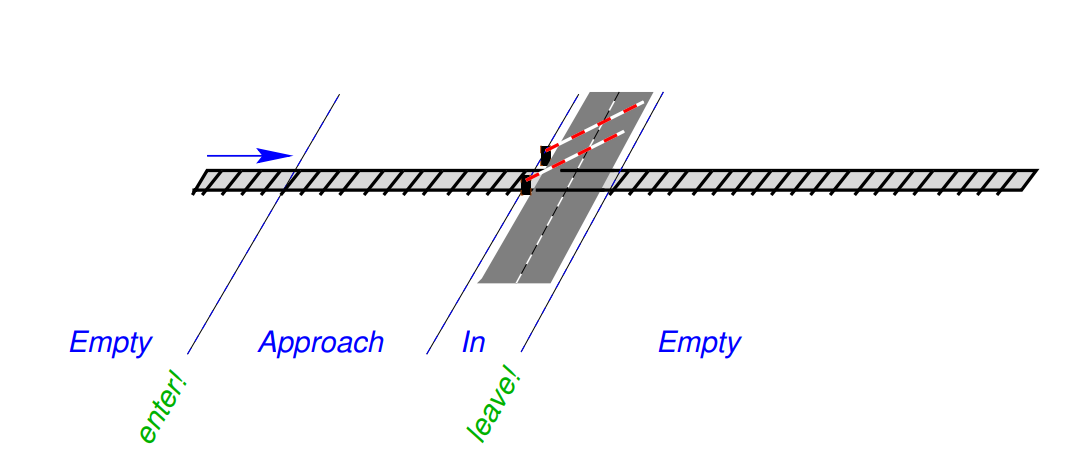
\includegraphics[scale=0.5]{train.png}

\noindent Dans ce cas de figure-ci, il est impératif que les portes soient fermées lorsque le train traverse le passage à niveau. Comme dit précédemment, un système informatique s'occupera de gérer cela.

\noindent Mais puisqu'on ne peut pas se permettre la moindre erreur, nous nous devons de vérifier que le système n'échouera jamais, et c'est dans ce cas de figure que le \textit{Model Checking} fut créé et utilisé.\\

\noindent Au cours de cette dissertation, nous passerons donc en revue chacun des points de vue qu'on peut adapter lorsqu'on parle de \textit{Model Checking CTL}.\\
Le premier point que nous aborderons sera l'aspect analytique du modèle (Qu'est-ce qu'on doit vérifier ?). Lors de ce chapitre, nous allons montrer la façon dont on découpe un système pour en faire des structures propice à l'analyse et à la vérification. Des structures comme les \textit{Kripke models} ou encore les arbre seront bien évidemment abordées. Une fois ces objets observés, nous étudierons la façon dont on peut vérifier l'efficacité d'un système.\\

\noindent Après avoir déterminer la façon dont on peut vérifier l'exactitude d'un système, nous évoquerons la consistance de telles méthodes. Nous prouverons donc de manière rigoureuse l'efficacité du \textit{Model Checking CTL}. \\

\noindent Enfin, nous aborderons la question algorithmique : Comment implémenter un tel modèle ? \\

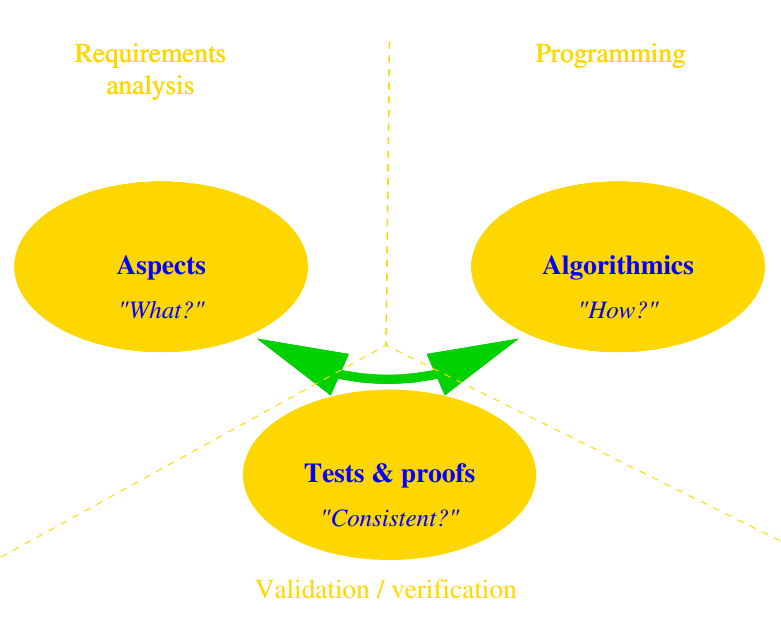
\includegraphics[scale=0.5]{points.png}

\noindent Il est évident que notre sujet ne s'arrêtera pas à ces points-ci. A titre d'exemple, nous comparerons également notre \textit{Model Checking CTL (Computational Tree Logic)} avec le \textit{LTL (Linear temporal logic)}.

\newpage

\section{Chapitre 1}
\subsection{Du graphe aux arbres de recherche}

Pour pouvoir analyser un système et pouvoir vérifier son efficacité, il est utile de le dériver en un graphe. Afin d'imager nos propos, reprenons l'exemple de la voie ferrée :\\ imaginons donc une voie ferrée sur laquelle aucun train ne circule. La voie est donc vide. On peut constate là un premier état de notre voie ferrée, l'état \textbf{vide}. Lorsque notre voie est vide, il se peut qu'à tout moment, un train soit \textbf{en approche}, et qu'on doive commencer à fermer les portes. Après quoi le train passera \textbf{sur} le passage à niveau pour ensuite repartir et laisser la voie \textbf{vide}.\\

\noindent Un tel système peut être représenté sous cette forme :  

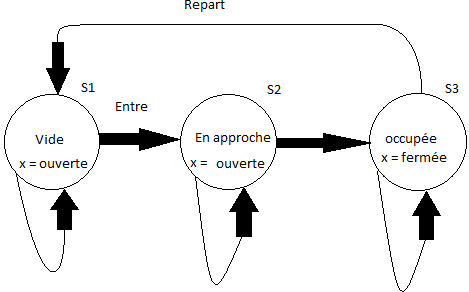
\includegraphics[scale=1]{graphe.png}

\noindent Avec x étant une variable d'état pour déterminer l'état des portes.\\

Nous avons donc ici un graphe infini puisque celui-ci est cyclique. lorsqu'on transformera ce graphe en un arbre de recherche, nous aurons donc également un arbre infini. Faisons le travail de transformer ce graphe en un arbre : 
\begin{center}
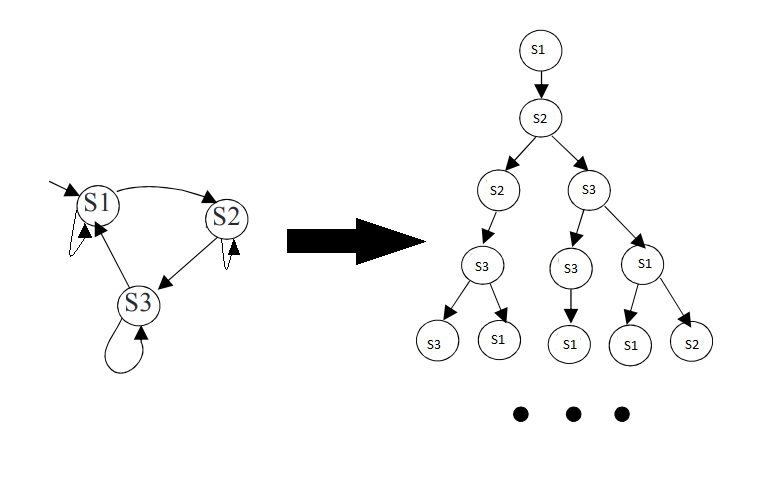
\includegraphics[scale=0.7]{kripke.png}
\end{center}

\noindent Les "..." symbolisent le fait le l'arbre est un arbre infini.\\

\noindent C'est maintenant grâce à de telles structures que nous allons pouvoir analyser notre système et vérifier que celui-ci soit infaillible.

 



\end{document}